
%!TeX program = lualatex
\documentclass[12pt]{article}

\usepackage[hmargin=0.5in, tmargin=0.75in, bmargin=0.9in]{geometry}
\geometry{legalpaper, portrait}

\usepackage{graphicx}  % graphic controls
\usepackage{float}  % positioning controls
\usepackage{lastpage}  % last page number finder
\usepackage{makecell}  % helpers for multilined table cells

% header/footer
\usepackage{fancyhdr}
\pagestyle{fancy}

\lhead{2023 June 5}
\chead{}
\rhead{\footnotesize \thepage \ {\color{gray} of \pageref{LastPage}}}

\cfoot{}
\rfoot{\textbf{\LARGE Congaree Activity Room Layout}\\\vspace{3pt}{\large\color{gray}NIH STTR Phase II}}

\renewcommand{\headrulewidth}{0.25pt}
\renewcommand{\footrulewidth}{0.25pt}

% drawing things
\usepackage{tikz}
\usetikzlibrary{math, calc, shapes, arrows.meta}

\tikzstyle{grid-line} = [gray, very thin]
\tikzstyle{wall} = [line width=2pt]
\tikzstyle{window} = [line width=1pt]
\tikzstyle{door} = [line width=1pt]
\tikzstyle{furniture} = [draw, line width=0.5pt, transform shape]
\tikzstyle{furniture-label} = [fill=white]
\tikzstyle{sensor} = [circle, draw, color=teal, fill=teal, inner sep=0.5mm]
\tikzstyle{sensor-label} = [above, yshift=2pt, fill=white, align=center, text=teal]
\tikzstyle{location} = [diamond, draw, color=violet, fill=violet, inner sep=0.5mm]
\tikzstyle{location-label} = [below, yshift=-3pt, fill=white, text=violet]
\tikzstyle{walking-path} = [densely dashed, line width=0.25mm, -{Stealth[length=4mm, width=2mm]}]
\tikzstyle{nav-arrow} = [line width=0.25mm, {Stealth[length=4mm, width=2mm]}-, green!60!black]
\tikzstyle{nav-arrow2} = [line width=0.25mm, {Stealth[length=4mm, width=2mm]}-, violet]

\tikzstyle{camera-label} = [fill=white, text=blue!75!black]

% units
\usepackage{siunitx}
\sisetup{per-mode = symbol}

\let\DeclareUSUnit\DeclareSIUnit
\let\US\SI
\let\us\si
\DeclareUSUnit\inch{in}
\DeclareUSUnit\feet{ft}
\DeclareUSUnit\foot{ft}
\DeclareUSUnit\pound{lb}
\DeclareUSUnit\slug{slug}

% paragraph settings
\setlength{\parindent}{0em}
\raggedright

\begin{document}
\vspace*{.8in}
\begin{figure}[H]
    \centering

    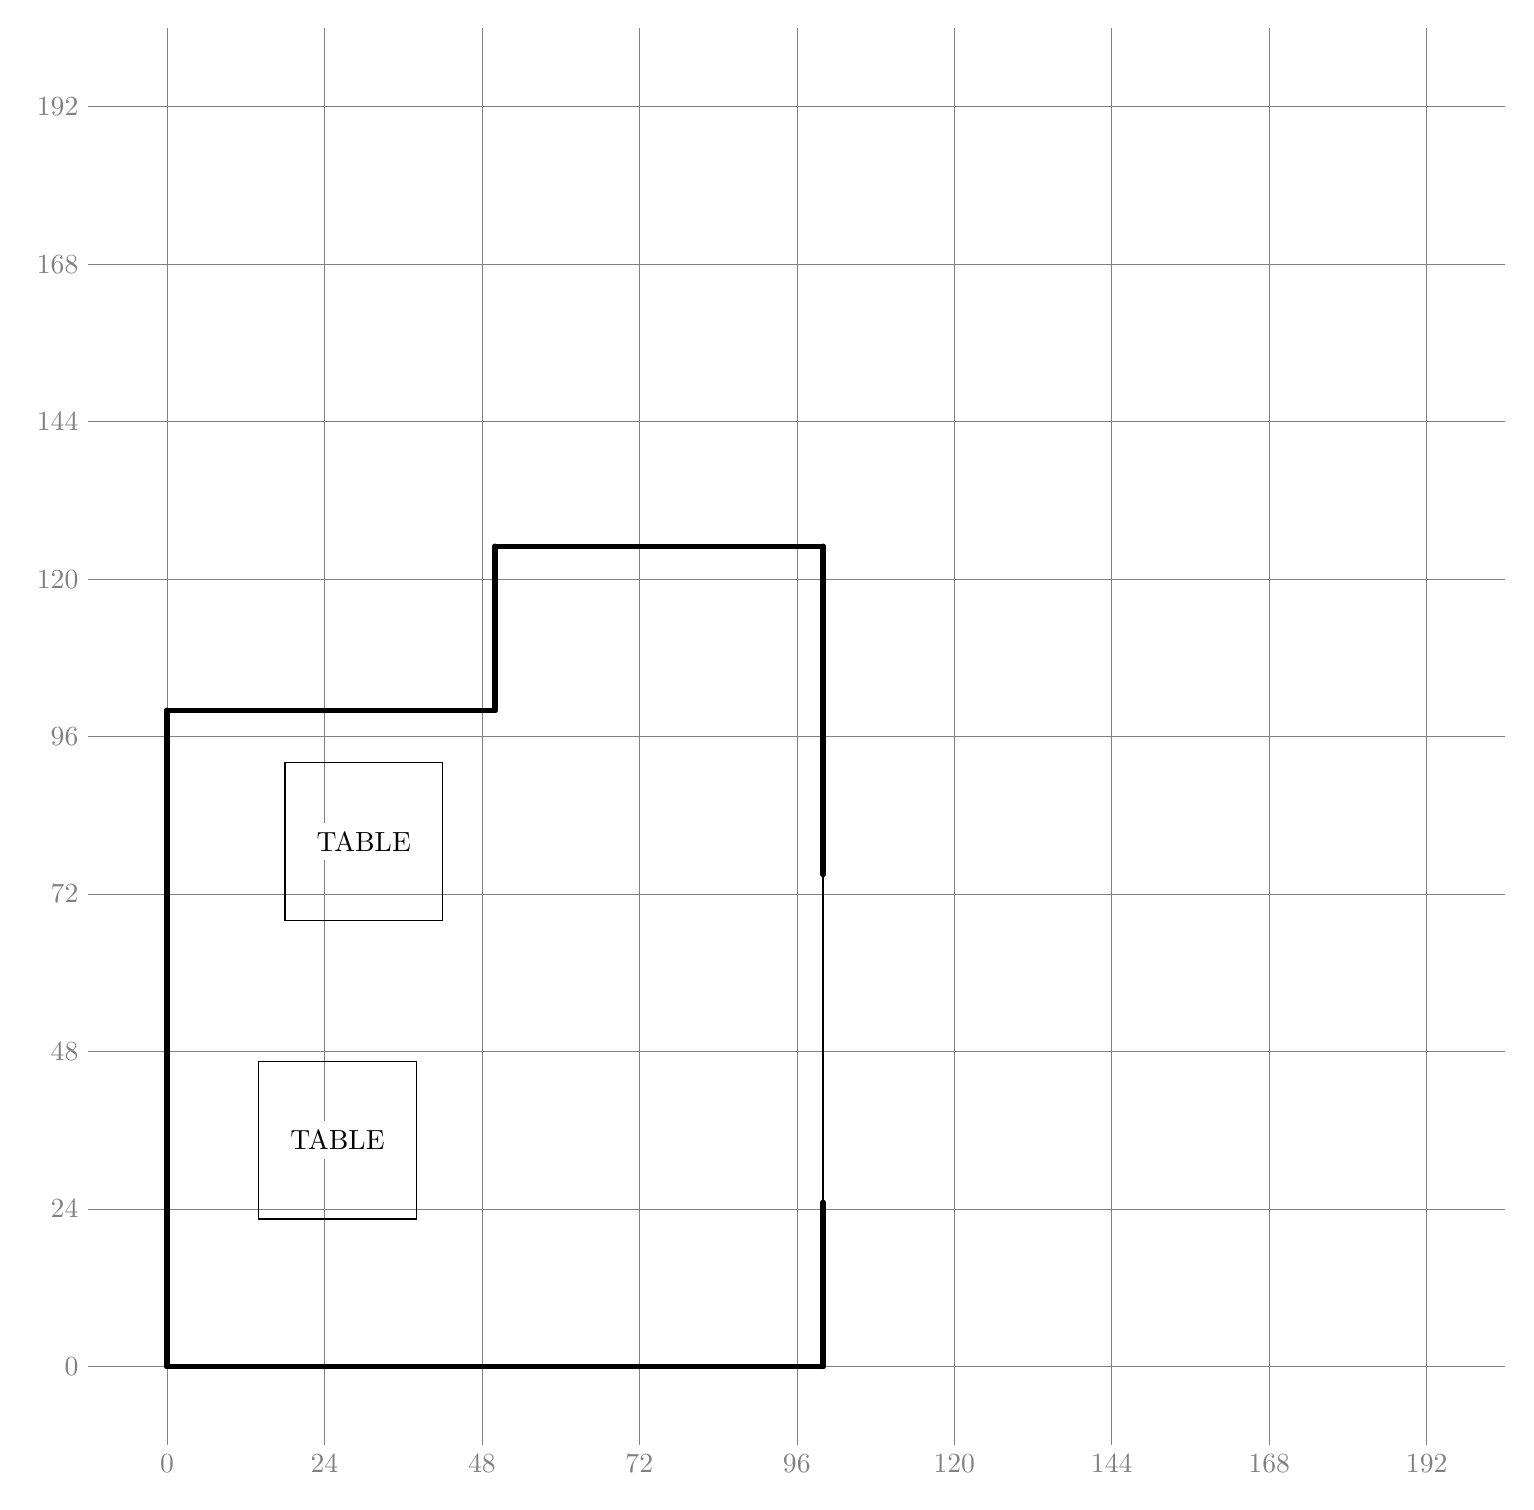
\begin{tikzpicture}[scale=1/12,  % use this to reduce or enlargen the image on paper
                        rotate=0]  % use this to rotate orientation by degrees on paper

    %% GRID - X
    \foreach \i in {0,24,...,192}{
        \draw[grid-line] (\i,-12) -- (\i,204);
        \tikzmath{int \value; \value = \i;}; 
        \node[gray, below] at (\i,-12) {\SI{\value}{\inch}};
    }

    %% GRID - Y
    \foreach \i in {0,24,...,192}{
        \draw[grid-line] (-12,\i) -- (204,\i);
        \tikzmath{int \value; \value = \i;};
        \node[gray, left] at (-12,\i) {\SI{\value}{\inch}};
    }

    \node[furniture, rectangle, minimum width=24.00cm, minimum height=24.00cm](table) at (26,34.5) {};
\node[furniture-label] at (table.center) {TABLE};
\node[furniture, rectangle, minimum width=24.00cm, minimum height=24.00cm](table) at (30,80.0) {};
\node[furniture-label] at (table.center) {TABLE};
\draw[wall, line cap=round] (0.00,0.00) -- (0.00,100.00) coordinate (c);
\draw[wall, line cap=round] (0.00,100.00) -- (50.00,100.00) coordinate (c);
\draw[wall, line cap=round] (50.00,100.00) -- (50.00,125.00) coordinate (c);
\draw[wall, line cap=round] (50.00,125.00) -- (100.00,125.00) coordinate (c);
\draw[wall, line cap=round] (100.00,125.00) -- (100.00,75.00) coordinate (c);
\draw[wall, line cap=round] (100.00,75.00) -- (100.00,75.00) coordinate (c);
\draw[window, line cap=round] (100.00,75.00) -- (100.00,25.00) coordinate (c);
\draw[window, line cap=round] (100.00,25.00) -- (100.00,25.00) coordinate (c);
\draw[wall, line cap=round] (100.00,25.00) -- (100.00,0.00) coordinate (c);
\draw[wall, line cap=round] (100.00,0.00) -- (0.00,0.00) coordinate (c);


    \end{tikzpicture}
\end{figure}
\end{document}
